\documentclass[a4paper,12pt,fleqn]{article}

% ============================================================
% 1. PACOTES ESSENCIAIS (CODIFICAÇÃO E IDIOMA)
% ============================================================

\usepackage[utf8]{inputenc}
\usepackage[T1]{fontenc}
\usepackage[brazilian]{babel} % Garante "Figura" e "Tabela" e hifenização PT-BR

% ============================================================
% 2. CONFIGURAÇÕES DE PÁGINA (GEOMETRIA E LAYOUT)
% ============================================================

%\usepackage{geometry}
%\geometry{
%	top=2.0cm, 
%	bottom=2.0cm, 
%	left=3cm, 
%	right=3cm, 
%	footskip=0.3cm % Distância do texto até o rodapé
%}

\usepackage{geometry}
\geometry{
	top=2.0cm,
	bottom=2.0cm,
	left=3cm,
	right=3cm,
	headheight=15pt, % Ajustado para evitar erro
	footskip=0.8cm   % Ajustado para evitar erro
}

\usepackage{setspace}
\setstretch{1.0}        % Espaçamento entre linhas 1.0
\singlespacing          % Garante espaçamento simples

\usepackage{multicol}   % Suporte a duas colunas
\usepackage{float}      % Controle de posicionamento [H]

\setlength{\columnsep}{0.8cm}

\usepackage{natbib}
\bibliographystyle{apalike}

% ============================================================
% 3. FONTES E MATEMÁTICA
% ============================================================

\usepackage{newtxtext}  % Fonte similar a Times New Roman
\usepackage{newtxmath}  % Fonte matemática compatível
\usepackage{amsmath}    % Comandos matemáticos avançados
\setlength{\mathindent}{0pt} % Equações alinhadas à esquerda (fleqn)

% ============================================================
% 4. CORES E ELEMENTOS GRÁFICOS
% ============================================================

\usepackage{xcolor}
\usepackage[table]{xcolor} % Cores em tabelas
\definecolor{verm}{RGB}{178, 34, 34} % Cor padrão ENEMP

\usepackage{graphicx}
\usepackage{eso-pic}    % Inserção de elementos no background (header)

% ============================================================
% 5. FORMATAÇÃO DE TABELAS
% ============================================================

\usepackage{booktabs}   % Réguas horizontais profissionais (\toprule, etc)
\usepackage{multirow}   % Mesclagem de linhas
\usepackage{makecell}   % Quebra de linha dentro de células
\usepackage{tabularx}   % Tabelas com largura ajustável

% ============================================================
% 6. CONFIGURAÇÃO DE LEGENDAS (CAPTION)
% ============================================================

\usepackage{caption}

% Configuração para Figuras
\captionsetup[figure]{
	labelsep=period, 
	justification=centering,
	font={normalsize}, 
	skip=10pt 
}

% Configuração para Tabelas
\captionsetup[table]{
	font={normalsize}, 
	labelsep=endash,
	justification=centering,
	skip=10pt
	%\renewcommand{\arraystretch}{1.5}
}

% ============================================================
% 7. FORMATAÇÃO DE TEXTO E PARÁGRAFOS
% ============================================================

\usepackage{ragged2e}   % Alinhamento justificado refinado
\usepackage{indentfirst} % Indenta o primeiro parágrafo das seções
\setlength{\parindent}{1.0cm}

\usepackage[none]{hyphenat} % Remove hifenização automática

% Controle de linhas órfãs e viúvas
\clubpenalty=10000
\widowpenalty=10000
\displaywidowpenalty=10000
\brokenpenalty=10000
\predisplaypenalty=10000
\postdisplaypenalty=10000

% ============================================================
% 8. TÍTULOS E LISTAS
% ============================================================

\usepackage{titlesec}
\titleformat{\section}{\normalfont\fontsize{12}{14}\bfseries}{\thesection}{1 em}{}
\titleformat{\subsection}{\normalfont\fontsize{12}{14}\bfseries}{\thesubsection}{1 em}{}
\titleformat{\subsubsection}{\normalfont\fontsize{12}{14}\bfseries\itshape}{\thesubsubsection}{1 em}{}
\setcounter{secnumdepth}{2}

\titlespacing*{\section}{0pt}{12pt}{0pt}
\titlespacing*{\subsection}{0pt}{12pt}{0pt}
\titlespacing*{\subsubsection}{0pt}{12pt}{0pt}

\usepackage{enumitem}
\setlist{
	noitemsep,     % Remove espaço entre itens
	topsep=0pt,    % Remove espaço antes da lista
	partopsep=0pt, 
	parsep=0pt     % Remove espaço entre parágrafos no item
}

% ============================================================
% 9. REFERÊNCIAS BIBLIOGRÁFICAS
% ============================================================

%\usepackage[alf, abnt-emphasize=bf, abnt-title-command=yes]{abntex2cite}

% ============================================================
% 10. CABEÇALHOS E RODAPÉS (FANCYHDR)
% ============================================================

\usepackage{fancyhdr}

% Estilo padrão para todas as páginas (exceto a primeira)
\pagestyle{fancy}
\fancyhf{} 
\renewcommand{\headrulewidth}{0.0pt} 
\fancyhead[C]{\fontsize{12}{14}\selectfont \color{verm} XLII Congresso Brasileiro de Sistemas Particulados (ENEMP)}
\fancyfoot[R]{\thepage}

% Estilo específico para a primeira página
\fancypagestyle{primeirapagina}{
	\fancyhf{}
	\renewcommand{\headrulewidth}{0pt}
	\fancyfoot[L]{%
		\fontsize{8}{9.6}\selectfont \color{verm}%
		Anais do ENEMP © 2026 ENEMP. \\%
		Esta é uma obra licenciada sob os termos da Licença CC BY-NC-SA 4.0.%
	}
	\fancyfoot[R]{\thepage}
}

% Inserção da imagem de cabeçalho na primeira página
\AddToShipoutPictureBG*{
	\AtPageUpperLeft{%
		\put(0,0){%
			\makebox(0,0)[lt]{%
				
\includegraphics[width=21cm, height=4.86cm, keepaspectratio=false]{image/header.jpg}%
			}%
		}%
	}
}

% ============================================================
% INÍCIO DO DOCUMENTO
% ============================================================

\begin{document}
	%\pagestyle{empty}
	% Espaço ajustado para o título começar após a imagem de 4,86cm
	\vspace*{2.5cm}

	% TÍTULO DO TRABALHO: Letras maiúsculas, negrito, centralizado, fonte 14
	\begin{center}
		{\bfseries\fontsize{14}{16}\selectfont TÍTULO DO TRABALHO}
	\end{center}

	% AUTORES: Inserir nomes completos. Máximo de 8 autores. Centralizado. Fonte 12.
	% Se for Student Contest, o candidato deve ser o primeiro autor.
	\begin{center}
		{\fontsize{12}{14}\selectfont João Pedro Câmara Borges$^{1*}$, João Paulo Colombo Lemes de Oliveira$^{1}$, Mauro Lúcio Naves Oliveira$^{1}$}
		
		\vspace{0.3cm}

		% FILIAÇÃO: Nome completo da instituição com endereço. Centralizado. Fonte 10.
		{\fontsize{10}{12}\selectfont
			$^{1}$Universidade Federal de Mato Grosso, Cuiabá-MT, Av. Fernando Correa da Costa, 2.367 – Boa Esperança \\
			*joao.borges2@sou.ufmt.br % Asterisco para indicar autor de correspondência
		}
	\end{center}

	\begin{justify}
		{\fontsize{12}{14}\selectfont
			\textbf{Resumo:} O resumo deve conter entre 100 e 200 palavras, abrangendo todos os pontos do trabalho, como motivação, objetivo, métodos adotados, principais resultados e conclusão. As palavras-chave devem seguir imediatamente abaixo do resumo, sendo de 3 a 5 palavras- -chave em letras minúsculas, separadas por ponto e vírgula e finalizadas por ponto. O título deve ser em negrito, com letras maiúsculas, centralizado, não excedendo 3 linhas. O nome dos autores deve ser escrito por extenso, separado por vírgula. Utilize um espaçamento de 12 pontos entre o título do trabalho e os autores. Os demais autores seguirão na sequência, sempre separados por ponto e vírgula. As afiliações devem ser indicadas por números arábicos sobrescritos ao final de cada autor, e cada afiliação correspondente deve ser escrita por extenso após a lista de autores. Utilize um espaçamento de 12 pontos entre os autores e as afiliações, e entre as afiliações e o resumo. O conteúdo referente a título, autores, resumo e abstract não pode ultrapassar uma página. \textbf{Todos os trabalhos submetidos ao student contest devem estar em inglês, exceto o resumo em português na primeira página. }

			\noindent
			\textbf{Palavras-chave:} primeiro termo; segundo termo; terceiro termo.}
	\end{justify}

	% TÍTULO DO TRABALHO EM INGLÊS: Letras maiúsculas, negrito, centralizado, fonte 14
	\begin{center}
		{\bfseries\fontsize{14}{16}\selectfont [TITLE IN ENGLISH] MODELO E INSTRUÇÕES PARA A ELABORAÇÃO DE TRABALHOS A SEREM SUBMETIDOS AO XLII CONGRESSO BRASILEIRO DE SISTEMAS PARTICULADOS}
	\end{center}

	% Abstract
	\begin{justify}
		{\fontsize{12}{14}\selectfont
			\textbf{Abstract:} As traduções para o inglês do título, do resumo (Abstract) e das palavras-chave (Keywords) devem ser apresentadas logo após o resumo. O trabalho deverá ter no mínimo 6 páginas e no máximo 10 páginas, não excedendo 2 MB em tamanho. O trabalho deve ser inédito, podendo ser do tipo original ou de revisão, e não deve ter sido apresentado anteriormente ou estar em processo de avaliação em outro evento, periódico ou qualquer outro meio de publicação. Será aceito um máximo de 08 autores por trabalho submetido, e não serão permitidas alterações na autoria (inclusões ou exclusões de autores) após a submissão efetiva. São aceitos trabalho nos idiomas português, espanhol ou inglês. Os autores são responsáveis pela autoria integral do texto, sem cópia, plágio ou equivalentes. O uso de inteligência artificial deve seguir a Política de Integridade na Atividade Científica do CNPq, de acordo com a portaria 2664/2026. O autor responsável pela submissão assume a responsabilidade de garantir que todos os autores estejam cientes do conteúdo do trabalho e de sua publicação na forma online em acesso aberto através dos anais do ENEMP.

			% Keywords
			\noindent
			\textbf{Keywords:} first keyword; second keyword; third keyword.
		}
	\end{justify}

	\thispagestyle{primeirapagina} %Rodapé

	\newpage %Nova pagina
	
	% =========================
	% INÍCIO DAS DUAS COLUNAS
	% =========================

	\newgeometry{
		top=2.0cm, 
		bottom=2.0cm, 
		left=2.0cm, 
		right=2.0cm, 
		footskip=1.0cm
	}

	\begin{multicols}{2}

		% =========================
		\section{Beneficiamento mineral}

			O beneficiamento mineral constitui uma etapa fundamental da cadeia produtiva da mineração, sendo responsável pela concentração dos minerais de interesse e pela redução da quantidade de material estéril destinado às etapas subsequentes do processo  (Wills e Finch, 2016). A eficiência dessa etapa está diretamente relacionada ao adequado projeto e operação das diversas operações unitárias empregadas no processamento do minério.

			A cadeia produtiva mineral compreende, de forma geral, as etapas de lavra, beneficiamento e disposição ou reaproveitamento dos rejeitos. No beneficiamento mineral, destacam-se operações como britagem, peneiramento, moagem, classificação, separação magnética, flotação, espessamento, filtragem e tratamento de rejeitos. Diversos equipamentos empregados nessas operações estão sujeitos a condições severas de desgaste devido ao processamento contínuo de polpas abrasivas, incluindo britadores, moinhos, bombas, tubulações, hidrociclones e sistemas de transporte hidráulico.

			Os principais mecanismos de degradação desses equipamentos incluem abrasão, impacto, erosão e corrosão, que frequentemente atuam de forma combinada. Para aumentar a vida útil dos equipamentos, empregam-se revestimentos cerâmicos e elastoméricos, ligas metálicas resistentes ao desgaste e revestimentos metálicos especiais, selecionados de acordo com as condições operacionais e as características da polpa processada.

			Os tanques de condicionamento são amplamente utilizados no beneficiamento mineral para promover a homogeneização da polpa com os reagentes químicos antes das etapas de separação, especialmente na flotação. Esses equipamentos são dotados de sistemas mecânicos de agitação compostos por impelidores, eixos e defletores, componentes que permanecem continuamente expostos ao contato com partículas abrasivas e meios quimicamente agressivos, tornando-se suscetíveis aos fenômenos de desgaste e corrosão. Além da flotação, tanques de condicionamento também são empregados em processos de lixiviação, neutralização e preparação de reagentes.

		\section{Misturador estático}
			Como alternativa aos tanques de condicionamento convencionais, os misturadores estáticos apresentam a vantagem de não possuírem partes móveis, reduzindo significativamente as necessidades de manutenção e aumentando sua confiabilidade operacional. Esses dispositivos utilizam a energia do próprio escoamento para promover a divisão, recombinação e mistura contínua de líquidos, gases e suspensões, sendo a perda de carga uma consequência do processo de mistura. Na indústria mineral, podem ser empregados no condicionamento contínuo de polpas e reagentes, na dispersão de gases, no ajuste de pH, no tratamento de água e efluentes e em outras operações de mistura em linha. Além disso, apresentam dimensões compactas e podem ser fabricados ou revestidos com materiais de elevada resistência à abrasão e à corrosão, tornando-os adequados para o processamento de polpas minerais.

			Para o presente trabalho estudou-se o comportamento hidrodinâmico do misturador estático com a presença de alguns elementos internos de mistura em termos da sua distribuição do tempo de residência. Isto para definir o quão bem o misturador estático pode ser utilizado com um tanque de condicionamento para futuros processos de flotação.

			\section{Experimento}
			O teste hidrodinâmico do misturador foi estudado a partir da introdução de elementos de mistura que dividem o aparelho em três secções. As combinações são: duas placas com furo centrado, dois cones posicionados com a concavidade voltada para cima e dois cones com a concavidade voltada para baixo. Outro parâmetro que adiciona combinações a serem estudadas é a velocidade do fluxo de água, variada pela modificação da potência das bombas de diafragma de alimentação. O planejamento do experimento para cada uma das configurações de elementos internos de mistura está disposto na Tabela \ref{tab:plan}.

		% Tabelas: legenda acima
		\begin{table}[H]
			\centering
			% Texto da tabela em tamanho 10 conforme solicitado
			\fontsize{10}{12}\selectfont 
			\caption{Planejamento experimental.}
			\label{tab:plan}

			% @{} remove os espaços nas pontas para alinhar perfeitamente com as margens
			% Use X, c, r ou l para adicionar colunas na tabela
			\begin{tabularx}{\columnwidth}{@{} >{\raggedright\arraybackslash}X r r r r @{}}
				\hline
				\addlinespace[0.2cm] % Espaço acima do texto do cabeçalho
				\textbf{Teste} & \textbf{\makecell{Bomba 1 \\ (\%)}} & \textbf{\makecell{Bomba 1 \\ (cod)}} & \textbf{\makecell{Bomba 2 \\ (\%)}} & \textbf{\makecell{Bomba 2 \\ (cod)}} \\
				\addlinespace[0.1cm] % Espaço acima do texto do cabeçalho
				\hline\addlinespace[0.2cm] % Espaço acima do texto
				01 & 50.0 & 0.00 & 50.0 & 0.00 \\
				02 & 7.6 & -1.66 & 50.0 & 0.00 \\
				03 & 80.0 & 1.00 & 80.0 & 1.00 \\
				04 & 20.0 & -1.00 & 80.0 & 1.00 \\
				% 05 & 50.0 & 0.00 & 50.0 & 0.00 \\
				06 & 20.0 & -1.00 & 20.0 & -1.00 \\
				% 07 & 50.0 & 0.00 & 50.0 & 0.00 \\
				08 & 50.0 & 0.00 & 92.4 & 1.66 \\
				% 09 & 50.0 & 0.00 & 50.0 & 0.00 \\
				10 & 50.0 & 0.00 & 7.6 & -1.66 \\
				% 11 & 50.0 & 0.00 & 50.0 & 0.00 \\
				% 12 & 50.0 & 0.00 & 50.0 & 0.00 \\
				13 & 92.4 & 1.66 & 50.0 & 0.00 \\
				14 & 80.0 & 1.00 & 20.0 & -1.00 \\
				% 15 & 50.0 & 0.00 & 50.0 & 0.00 \\
				\hline
			\end{tabularx}
		\end{table}

		\section{Montagem do sistema}
			A montagem do sistema é baseada na presença de quatro bombas de diafragma para transporte da água de diluição, duas bombas peristalticas para injeção do traçador em pulso de 40 cts, dois tanques de água, um tanque de recalque, um tanque de mistura, duas valvulas solenoide que leva água ou para o tanque reservatório interno ou para o tanque de recalque e um medidor de concentração na saida do misturador, a Figura \ref{fig:system} exemplifica a montagem do sistema.

			\begin{figure}[H]
				\centering
				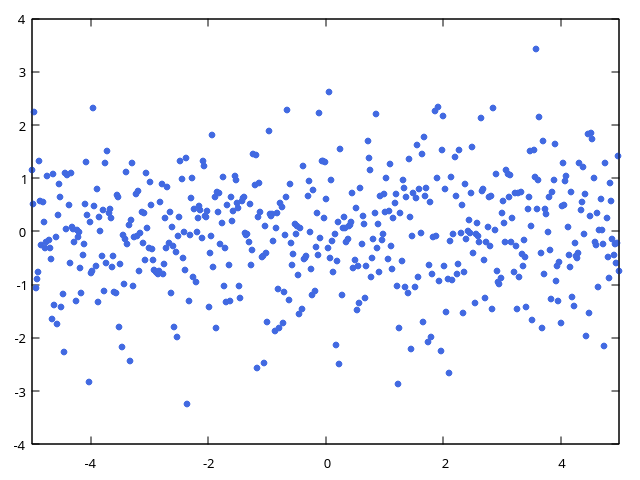
\includegraphics[width=\columnwidth]{image/figura.png}
				\caption{Esquemático da montagem do sistema.}
				\label{fig:system}
			\end{figure}

			Segundo essa configuração, a medição da concentração no tanque de mistura funciona como um vaso fechado, ou seja, uma caixa preta e que o estudo da fluiodinâmica é inteiramente baseado na interpretação dos dados de concentração de saida, isso em função do posicionamento ou geometria dos elementos internos.

		\section{Tratamento de Dados}
			Os dados de estímulo resposta são convertidos para concentração dentro do algoritmo em python, a partir disso é possível graficar valores de concentração por tempo. Esses valores são utilizados na parametrização da Equação \ref{eq:distribution}, que possui os parâmetros N e tau \citep{levenspiel}.

			\begin{equation}
				E(\theta) = \frac{N (N \theta)^{N - 1}}{(N - 1)!} e^{-N \theta}
				\label{eq:distribution}
				% \frac{\partial C}{\partial t} = \dfrac{D}{r}\dfrac{\partial D}{\partial r}+ \frac{\partial^2 C}{\partial t^2},
			\end{equation}

			% Definir símbolos na primeira ocorrência

			\noindent onde:\\
			\begin{tabularx}{\columnwidth}{@{} l X r @{}}
				$\theta$ & Tempo adimensional & \\
				$E(\theta)$ & Fração de traçador em $\theta$ & \\
				$N$ & Número correspondente de tanques & \\
			\end{tabularx}

			O algoritmo de ajuste se baseia na redução dos erros quadráticos ponderados pelo tempo, portanto, valores de N entre $1$ e $2$ e os valores de tempo médio $\tau$ entre $50$ e $400$ s são testados e a combinação que atinge o valor mínimo do erro é considerada a melhor opção. O intervalo de teste de N e $\tau$ são heurísticas baseadas no entendimento do sistema.

			A precisão dos resultados é incrementada pela expansão dos valores adjacentes ao mínimo encontrado. Tanto para N quanto para tau, a diminuição da diferença entre valores sucessivos é dada por um fator de $100$, isso é feito quatro vezes, porque a partir dessa quantidade de iterações o progresso é notavelmente pequeno. A utilização deste método de segmentação aumentada do intervalo de interesse é possível e necessária dada a natureza da equação ajustada, para que o resultado da aproximação pela curva não dependa dos chutes iniciais.

		\section{Resultados}
			As curvas de distribuição do tempo de residência adimensional, em resposta à pertubação em pulso tem seu formato característico como mostrado na Figura \ref{fig:plate_raw_curve}, onde há um pico de passagem de traçador na saída do misturador logo no início do experimento. Vale notar tambem que o gráfico não exibe atraso, em parte, esse comportamento se deve pelo projeto cuidadoso do reator que minimiza o atraso, mas o fator que melhor explica esse fenômeno é a arbitrariedade da escolha do ínicio da curva para o momento da iminência da sua evolução, visando o estudo da distribuição dos reagentes pelo ajuste da Equação \ref{eq:distribution}.

			\begin{figure}[H]
				\centering
				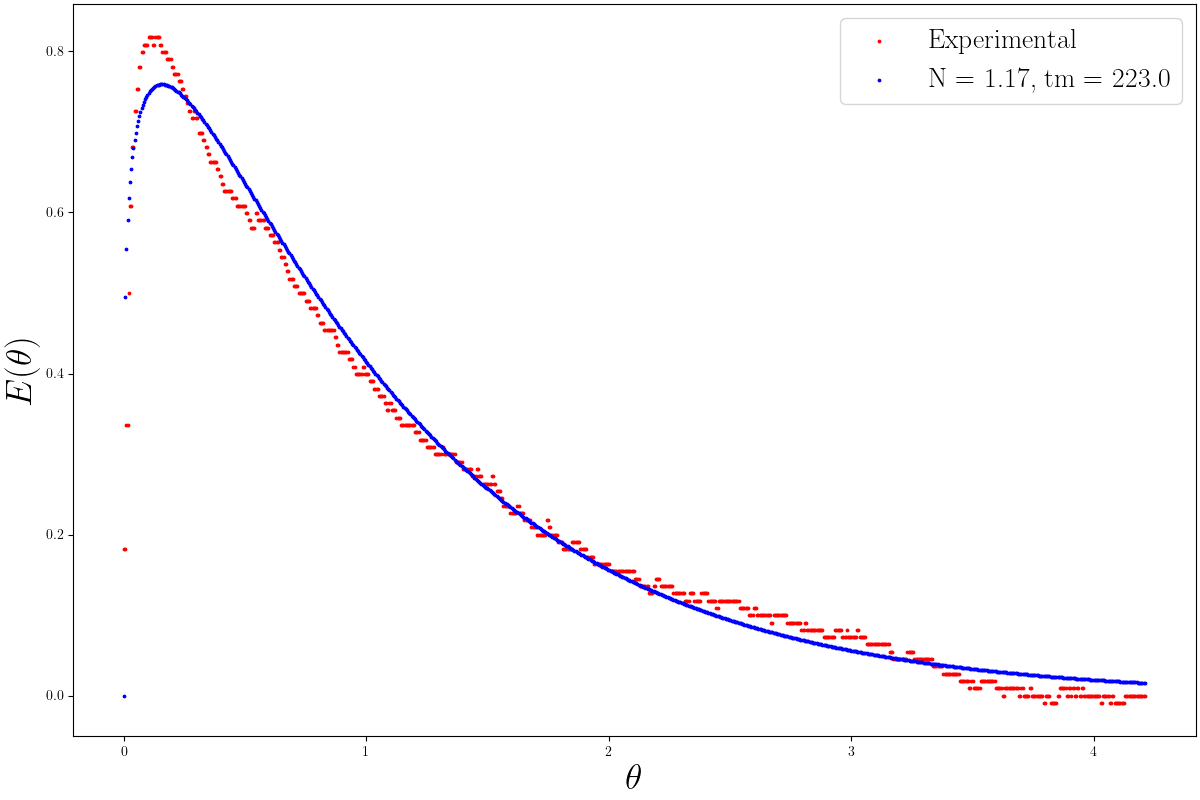
\includegraphics[width=\columnwidth]{image/01_plate.png}
				\caption{Concentração por tempo na saida do misturador para a primeira rodada do planejamento experimental com potências de bombas medianas e placa com furo central como elemento interno de mistura.}
				\label{fig:plate_raw_curve}
			\end{figure}

			Na configuração do primeiro teste do planejamento experimental, o misturador tem um comportamento proximo de um reator de mistura ideal \citep{levenspiel}, ou melhor, sua proximidade com um reator de mistura ideal é maior que a das configurações com as mesmas potências de bombas, mas com diferentes elementos de mistura, sendo que o cone com concavidade para cima (Figura \ref{fig:down_first_curve}) teve um resultado ligeiramente melhor que o teste do cone voltado para baixo (Figura \ref{fig:up_raw_curve}). Tudo isso para a vazão intermediária do planejamento.

			\begin{figure}[H]
				\centering
				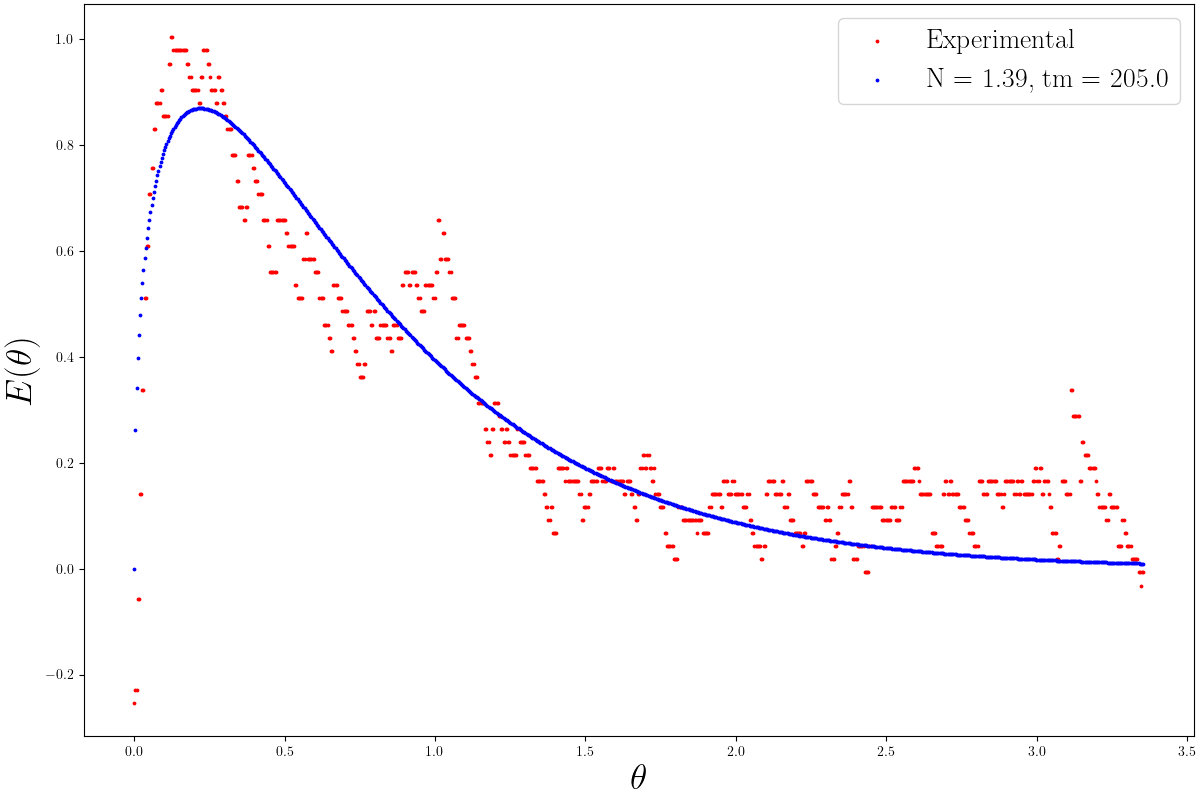
\includegraphics[width=\columnwidth]{image/01_down.png}
				\caption{Concentração por tempo na saida do misturador para a primeira rodada do planejamento experimental com potências de bombas medianas e cone voltado para baixo como elemento interno de mistura.}
				\label{fig:down_raw_curve}
			\end{figure}

			\begin{figure}[H]
				\centering
				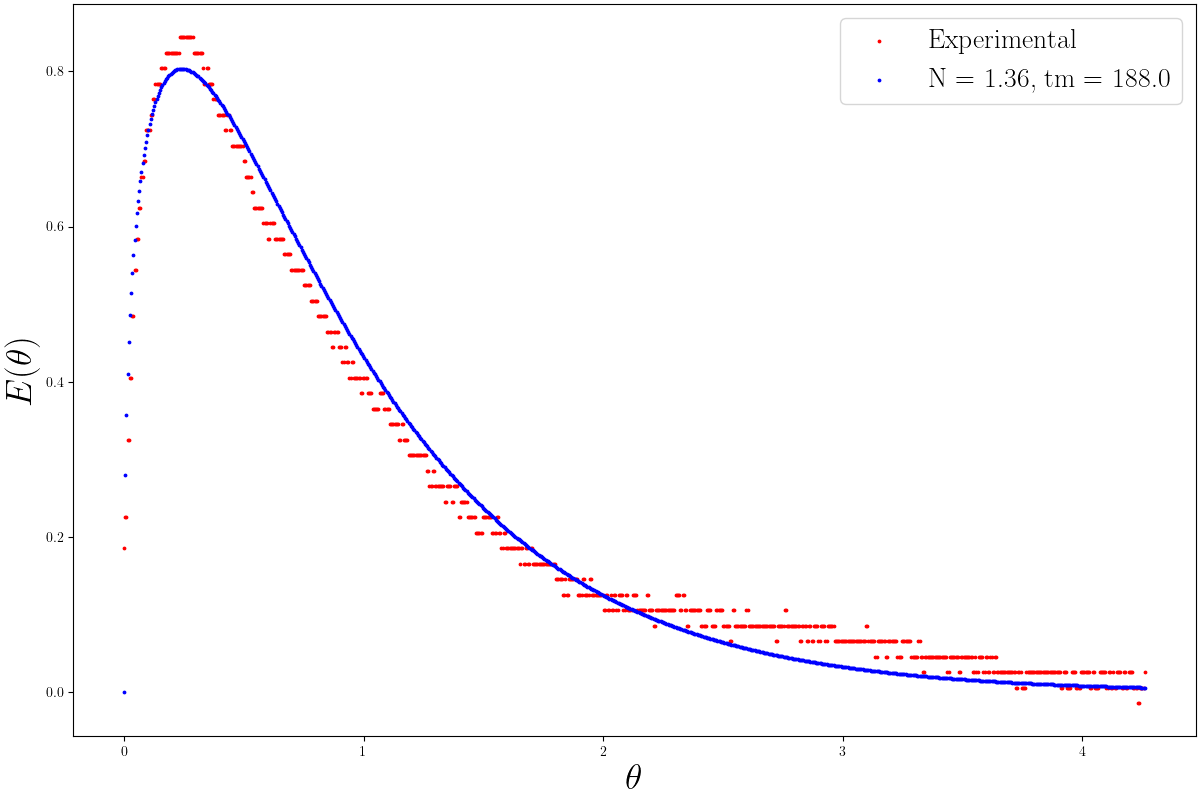
\includegraphics[width=\columnwidth]{image/01_up.png}
				\caption{Concentração por tempo na saida do misturador para a primeira rodada do planejamento experimental com potências de bombas medianas e cone voltado para cima como elemento interno de mistura.}
				\label{fig:up_raw_curve}
			\end{figure}

			Pode-se ver, ainda nos primeiros experimentos que existe uma diferênça nas dispersões axiais de cada uma das configurações. Isto é visto a partir da analise da variância em uma analise quantitativa, ou a partir da observação da largura da curva. A ordem de dispersão axial por padrões visuais da maior para a menor é placa, cone para cima e cone para baixo respectivamente.

			A configuração com cone para baixo tem uma dispersão axial menor que as outras alternativas, isso é facilmente visualizado a partir estabilidade de sua calda, percebe-se que ela não asume uma direção na segunda metade do experimento. Essa estabilidade, ou até mesmo o comportamento geral do experimento com cone para baixo são mascarados pela variabilidade dos pontos experimentais que não aparentam terem um comportamento suave.

		\section{Conclusão}

	% ============================================================
	% REFERÊNCIAS
	% ============================================================
	\section*{Referências}
	\begingroup
	\renewcommand{\section}[2]{} 

	\makeatletter
	% MÁGICA QUE APAGA O NOME DUPLICADO (Esconde o rótulo)
	\renewcommand{\@biblabel}[1]{}

	% REESCREVE A BIBLIOGRAFIA PARA ZERAR QUALQUER RECUO
	\renewenvironment{thebibliography}[1]{%
		\list{}{%
			\setlength{\leftmargin}{0pt}  % Zera a margem esquerda de todas as linhas
			\setlength{\itemindent}{0pt}  % Zera o recuo da primeira linha
			\setlength{\labelwidth}{0pt}  % Zera o espaço oculto do rótulo
			\setlength{\labelsep}{0pt}    % Zera a separação do rótulo
			\setlength{\itemsep}{10pt}    % Mantém os 10pt entre cada referência
			\setlength{\parsep}{0pt}
		}%
		\sloppy      % Força justificação sem vazar a margem
		\justifying  % Garante o alinhamento justificado
	}{%
		\endlist
	}
	\makeatother

	\fontsize{10}{12}\selectfont

	% Usa apalike
	\bibliography{main}
	\endgroup

	\end{multicols}
\end{document}
